\documentclass[aspectratio=169]{beamer}
\usepackage{tikz}
\usepackage{newpxmath, newpxtext}
\usepackage{amsmath}
\usepackage{color}
\usefonttheme[]{serif}
\newcommand{\bvec}[1]{\mbox{\boldmath $#1$}}


\title{Numerical Calculation of 1-d Dimensional Heat Equation by explicit method}
\author{Taro Morita}

\begin{document}
\begin{frame}
    \titlepage
\end{frame}

\begin{frame}
    \frametitle{Heat Equation}
    \framesubtitle{Explicit method}
    \begin{equation}
        \frac{\partial \theta}{\partial t} = \kappa \frac{\partial^2 \theta}{\partial x^2}
    \end{equation}
    Recurrence formula is ...
    \begin{equation}
        \frac{\theta_{i, j+1} - \theta_{i, j}}{\Delta t} = \kappa \frac{\theta_{i-1, j} - 2 \theta_{i, j} + \theta_{i+1, j}}{(\Delta x)^2}
        \label{eq:2}
    \end{equation}
\end{frame}

\begin{frame}
    \frametitle{Heat equation}
    \framesubtitle{Explicit method}
    Transforming equation \ref{eq:2}, we get
    \begin{equation}
        \theta_{i, J+i} = r \theta_{i-1, j} + (1 - 2 r) \theta_{i, j} + r \theta_{i-1, j}
    \end{equation}
    Where $r = \kappa \displaystyle{\frac{\Delta t}{(\Delta x)^2}}$
\end{frame}

\begin{frame}
    \frametitle{Heat equation}
    \framesubtitle{Explicit method}
    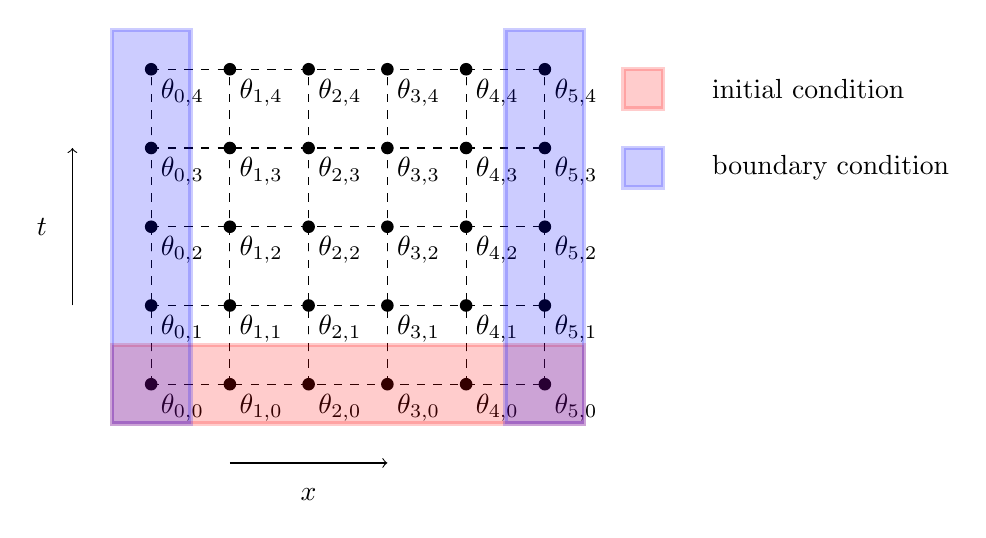
\begin{tikzpicture}
        \centering

        \foreach \y in {0, 1, ..., 4}
        {
            \draw [dashed] (0,\y) -- (5,\y);
            \foreach \x in {0, 1, ..., 5} 
            {
                \draw [dashed] (\x,0) -- (\x,4);
                \fill (\x,\y) circle [radius=0.08];
                \coordinate [label=below right:$\theta_{\x, \y}$] (0) at (\x, \y);
            }

        }
        \draw[->] (1,-1) -- (3, -1);
        \draw[->] (-1, 1) -- (-1, 3);
        \coordinate [label=below : $x$] (x) at (2, -1.2);
        \coordinate [label=left : $t$] (t) at (-1.2, 2);
        \draw [ultra thick, draw=red, fill=red, opacity=0.2] (-0.5, -0.5) -- (5.5, -0.5) -- (5.5, 0.5) -- (-0.5, 0.5)--cycle;
        \draw [ultra thick, draw=blue, fill=blue, opacity=0.2] (-0.5, -0.5) -- (0.5, -0.5) -- (0.5, 4.5) -- (-0.5, 4.5)--cycle;
        \draw [ultra thick, draw=blue, fill=blue, opacity=0.2] (4.5, -0.5) -- (5.5, -0.5) -- (5.5, 4.5) -- (4.5, 4.5)--cycle;
        \draw [ultra thick, draw=red, fill=red, opacity=0.2] (6, 3.5) -- (6.5, 3.5) -- (6.5, 4) -- (6, 4)--cycle;
        \draw [ultra thick, draw=blue, fill=blue, opacity=0.2] (6, 2.5) -- (6.5, 2.5) -- (6.5, 3) -- (6, 3)--cycle;
        \coordinate [label=right: initial condition] (I) at (7,3.75);
        \coordinate [label=right: boundary condition] (I) at (7,2.75);
    \end{tikzpicture}
\end{frame}

\begin{frame}
    \frametitle{Heat equation}
    \framesubtitle{Initial condition and boundary condition}
    \begin{block}{Initial condition}
        $\theta_{i, 0}$: initial temperature of the conductor
    \end{block}
    \begin{block}{Boundary condition}
        $\theta_{0, j}$, $\theta_{n, j}$: boundary temperature of the conductor ($n$: last element)
    \end{block}
\end{frame}

\begin{frame}
    \frametitle{Heat equation}
    \framesubtitle{Initial condition and boundary condition}
    \begin{block}{Example}
        \textcolor{red}{Put 300\textdegree C soldering iron on left side} of the metal \textcolor{red}{at room temperature (20\textdegree C)} , and \textcolor{red}{the right side was released.}
    \end{block}
    \begin{itemize}
        \item Initial condition $\theta_{i, 0}$ : 20~\textdegree C
        \item Boundary condition (left side) $\theta_{0, j}$ : 300~ \textdegree C
        \item Boundary condition (right side) $\theta_{n, j}$ : 20~ \textdegree C
    
    \end{itemize}
\end{frame}

\begin{frame}
    \frametitle{Heat equation}
    \begin{columns}
        \begin{column}{.48\linewidth}
            \begin{block}{$j = 0$}
                $i = 1$ :\\
                \begin{center}
                    $\theta_{1, 1} = r \theta_{0, 0} + (1-2r)\theta_{1, 0} + r \theta_{2, 0}$\\
                \end{center}
                $i = 2$ : \\
                \begin{center}
                    $\theta_{2, 1} = r \theta_{1, 0} + (1-2r)\theta_{2, 0} + r \theta_{3, 0}$\\
                \end{center}
                $i = 3$ : \\
                \begin{center}
                    $\theta_{3, 1} = r \theta_{2, 0} + (1-2r)\theta_{3, 0} + r \theta_{4, 0}$\\
                \end{center}
                $i = 4$ : \\
                \begin{center}
                    $\theta_{4, 1} = r \theta_{3, 0} + (1-2r)\theta_{4, 0} + r \theta_{5, 0}$\\
                \end{center}

            \end{block}
        \end{column}

        \begin{column}{.48\linewidth}
           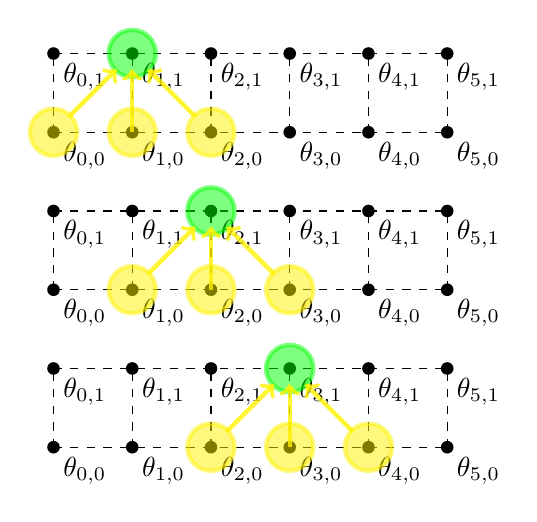
\begin{tikzpicture}
            \foreach \n in {1, 3, 5}
            {

                \foreach \y in {0, 1}
                {
                    \draw [dashed] (0, \y-\n) -- (5, \y-\n);
                    \foreach \x in {0, 1, 2, ..., 5}
                    {
                        \draw [dashed] (\x, -\n) -- (\x, 1-\n);
                        \fill (\x,\y-\n) circle [radius=0.08];
                        \coordinate [label=below right:$\theta_{\x, \y}$] (0) at (\x, \y-\n);
                    }
                }
                \draw [ultra thick, draw=green, fill=green, opacity=0.5, ] (\n/2+1/2,1-\n) circle [radius=0.3];
                \draw [ultra thick, draw=yellow, fill=yellow, opacity=0.5, ] (\n/2+1/2-1,-\n) circle [radius=0.3];
                \draw [ultra thick, draw=yellow, fill=yellow, opacity=0.5, ] (\n/2+1/2,-\n) circle [radius=0.3];
                \draw [ultra thick, draw=yellow, fill=yellow, opacity=0.5, ] (\n/2+1/2+1,-\n) circle [radius=0.3];
                \draw [->, ultra thick, draw=yellow, opacity=0.8] (\n/2+1/2-0.8,0.2-\n) -- (\n/2+1/2-0.2,0.8-\n);
                \draw [->, ultra thick, draw=yellow, opacity=0.8] (\n/2+1/2,-\n) -- (\n/2+1/2,0.8-\n);
                \draw [->, ultra thick, draw=yellow, opacity=0.8] (\n/2+1/2+0.8,0.2-\n) -- (\n/2+1/2+0.2,0.8-\n);

            }
               
           \end{tikzpicture} 
        \end{column}
    \end{columns}
\end{frame}

\begin{frame}
    \frametitle{Heat equation}
    \framesubtitle{Matrix}
    \begin{equation}
        \begin{pmatrix}
            \bvec{\theta_{0, k+1}} \\
            \bvec{\theta_{1, k+1}} \\
            \bvec{\theta_{2, k+1}} \\
            \bvec{\theta_{3, k+1}} \\
            \vdots \\
            \bvec{\theta_{n, k+1}} \\
        \end{pmatrix}
         = 
        \begin{pmatrix}
            1 - 2r & r & 0 & 0 & \cdots & 0 \\
            r & 1 - 2r & r & 0 & \cdots & 0 \\
            0 & r & 1 - 2r & r & \cdots & 0 \\
            0 & 0 & r & 1 - 2r & r & \vdots \\
            \vdots & & & & \ddots \\
            0 & \cdots & & & r & 1 
        \end{pmatrix}
        \begin{pmatrix}
            \bvec{\theta_{0, k}} \\
            \bvec{\theta_{1, k}} \\
            \bvec{\theta_{2, k}} \\
            \bvec{\theta_{3, k}} \\
            \vdots \\
            \bvec{\theta_{n, k}} \\
            
        \end{pmatrix}
    \end{equation}

    \vspace{5mm}
    \centering
    Calculate temperature at next step using temperature at current step
\end{frame}
\end{document}
